% !TEX root = ../../main.tex

% --------------------------------------
% labels: \label{mil4:res:[type]:[name]}
% --------------------------------------
% PAST TENSE



\begin{figure}[!ht]
    \centering
    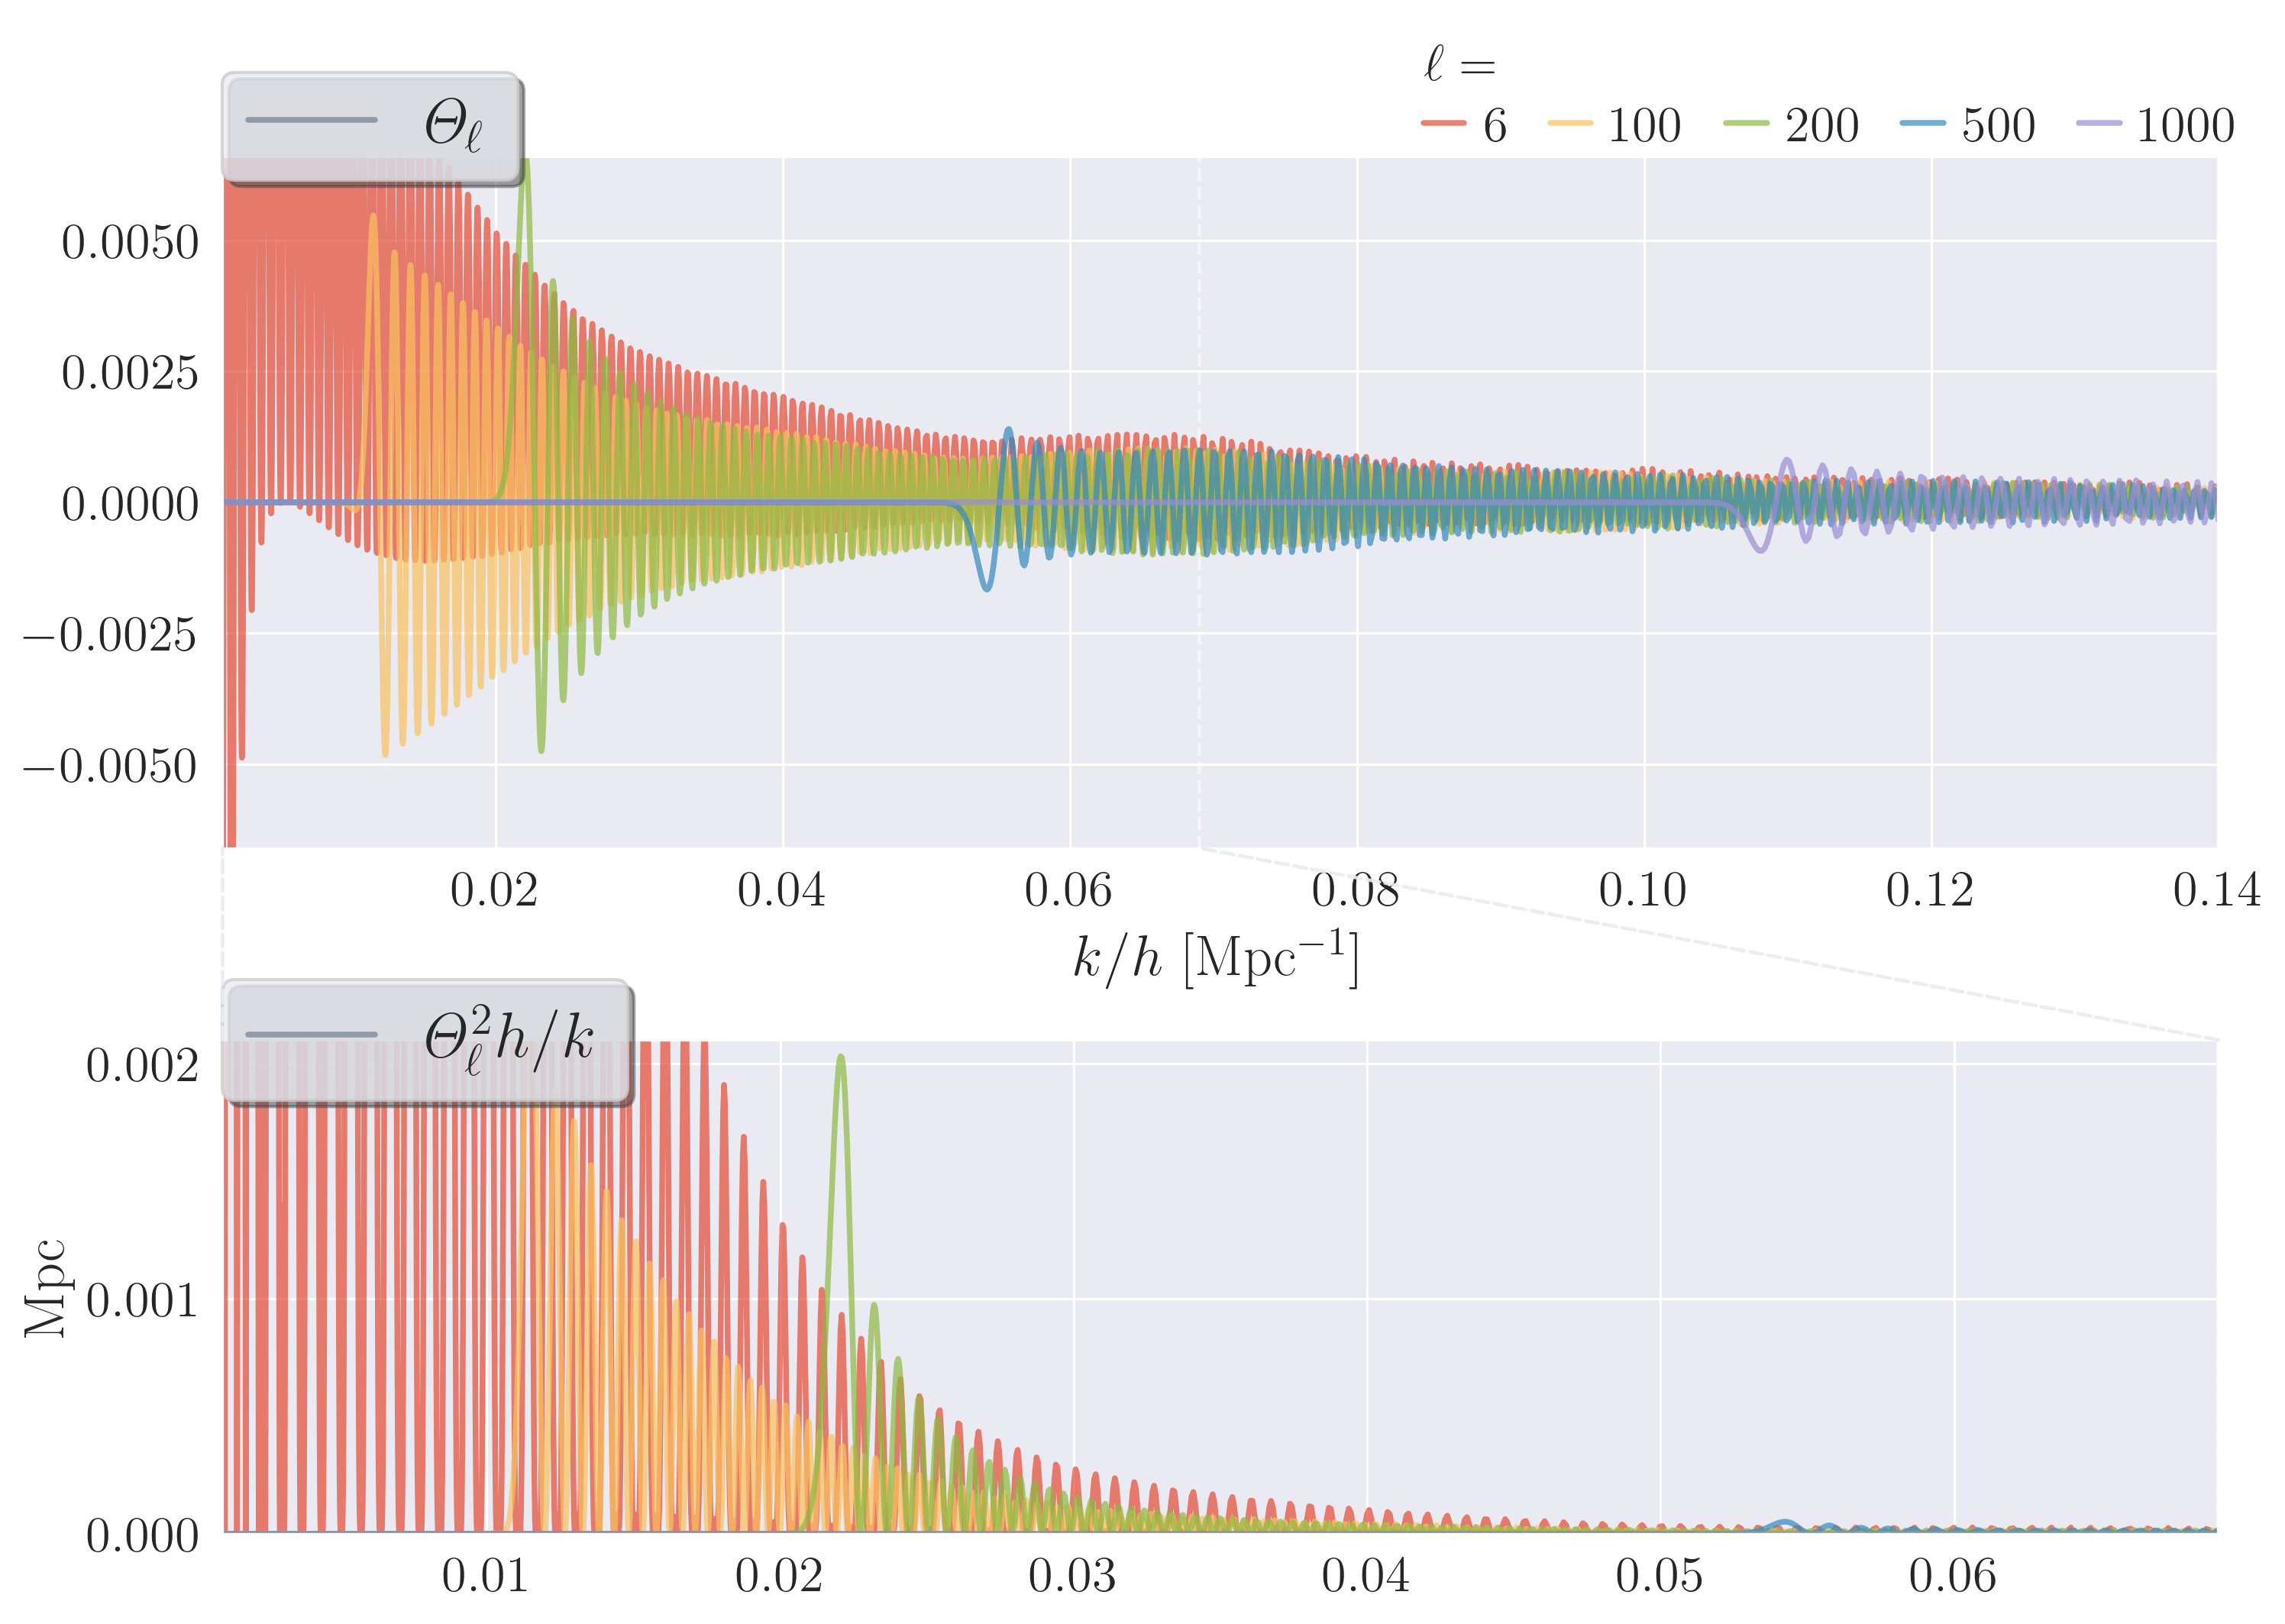
\includegraphics[width=\linewidth]{milestone4/Theta_ell.png} 
    \caption{The photon transfer functions $\Theta_\ell(x_0, k)$ as functions of wavenumber $k$ for a set of $\ell$s. Upper panel: Plainly $\Theta_\ell(0, k)$. Lower panel: Squared and scaled $\frac{\Theta^2_\ell(0,k)}{k}$.} 
\label[fig]{mil4:res:fig:transfer}
\end{figure}

The CMB power spectrum is presented in~\cref{mil4:res:fig:CMB_power}. The different contributions to the CMB anisotropy were overplotted, as well as the cosmic variance. We included observational data from~\citet{Planckdata} for low $\ell$. Observational data become less relevant for $\ell \gtrsim 200$ as effects of e.g.\ neutrinos are non-negligible at these scales.
\begin{figure}[!ht]
    \centering
    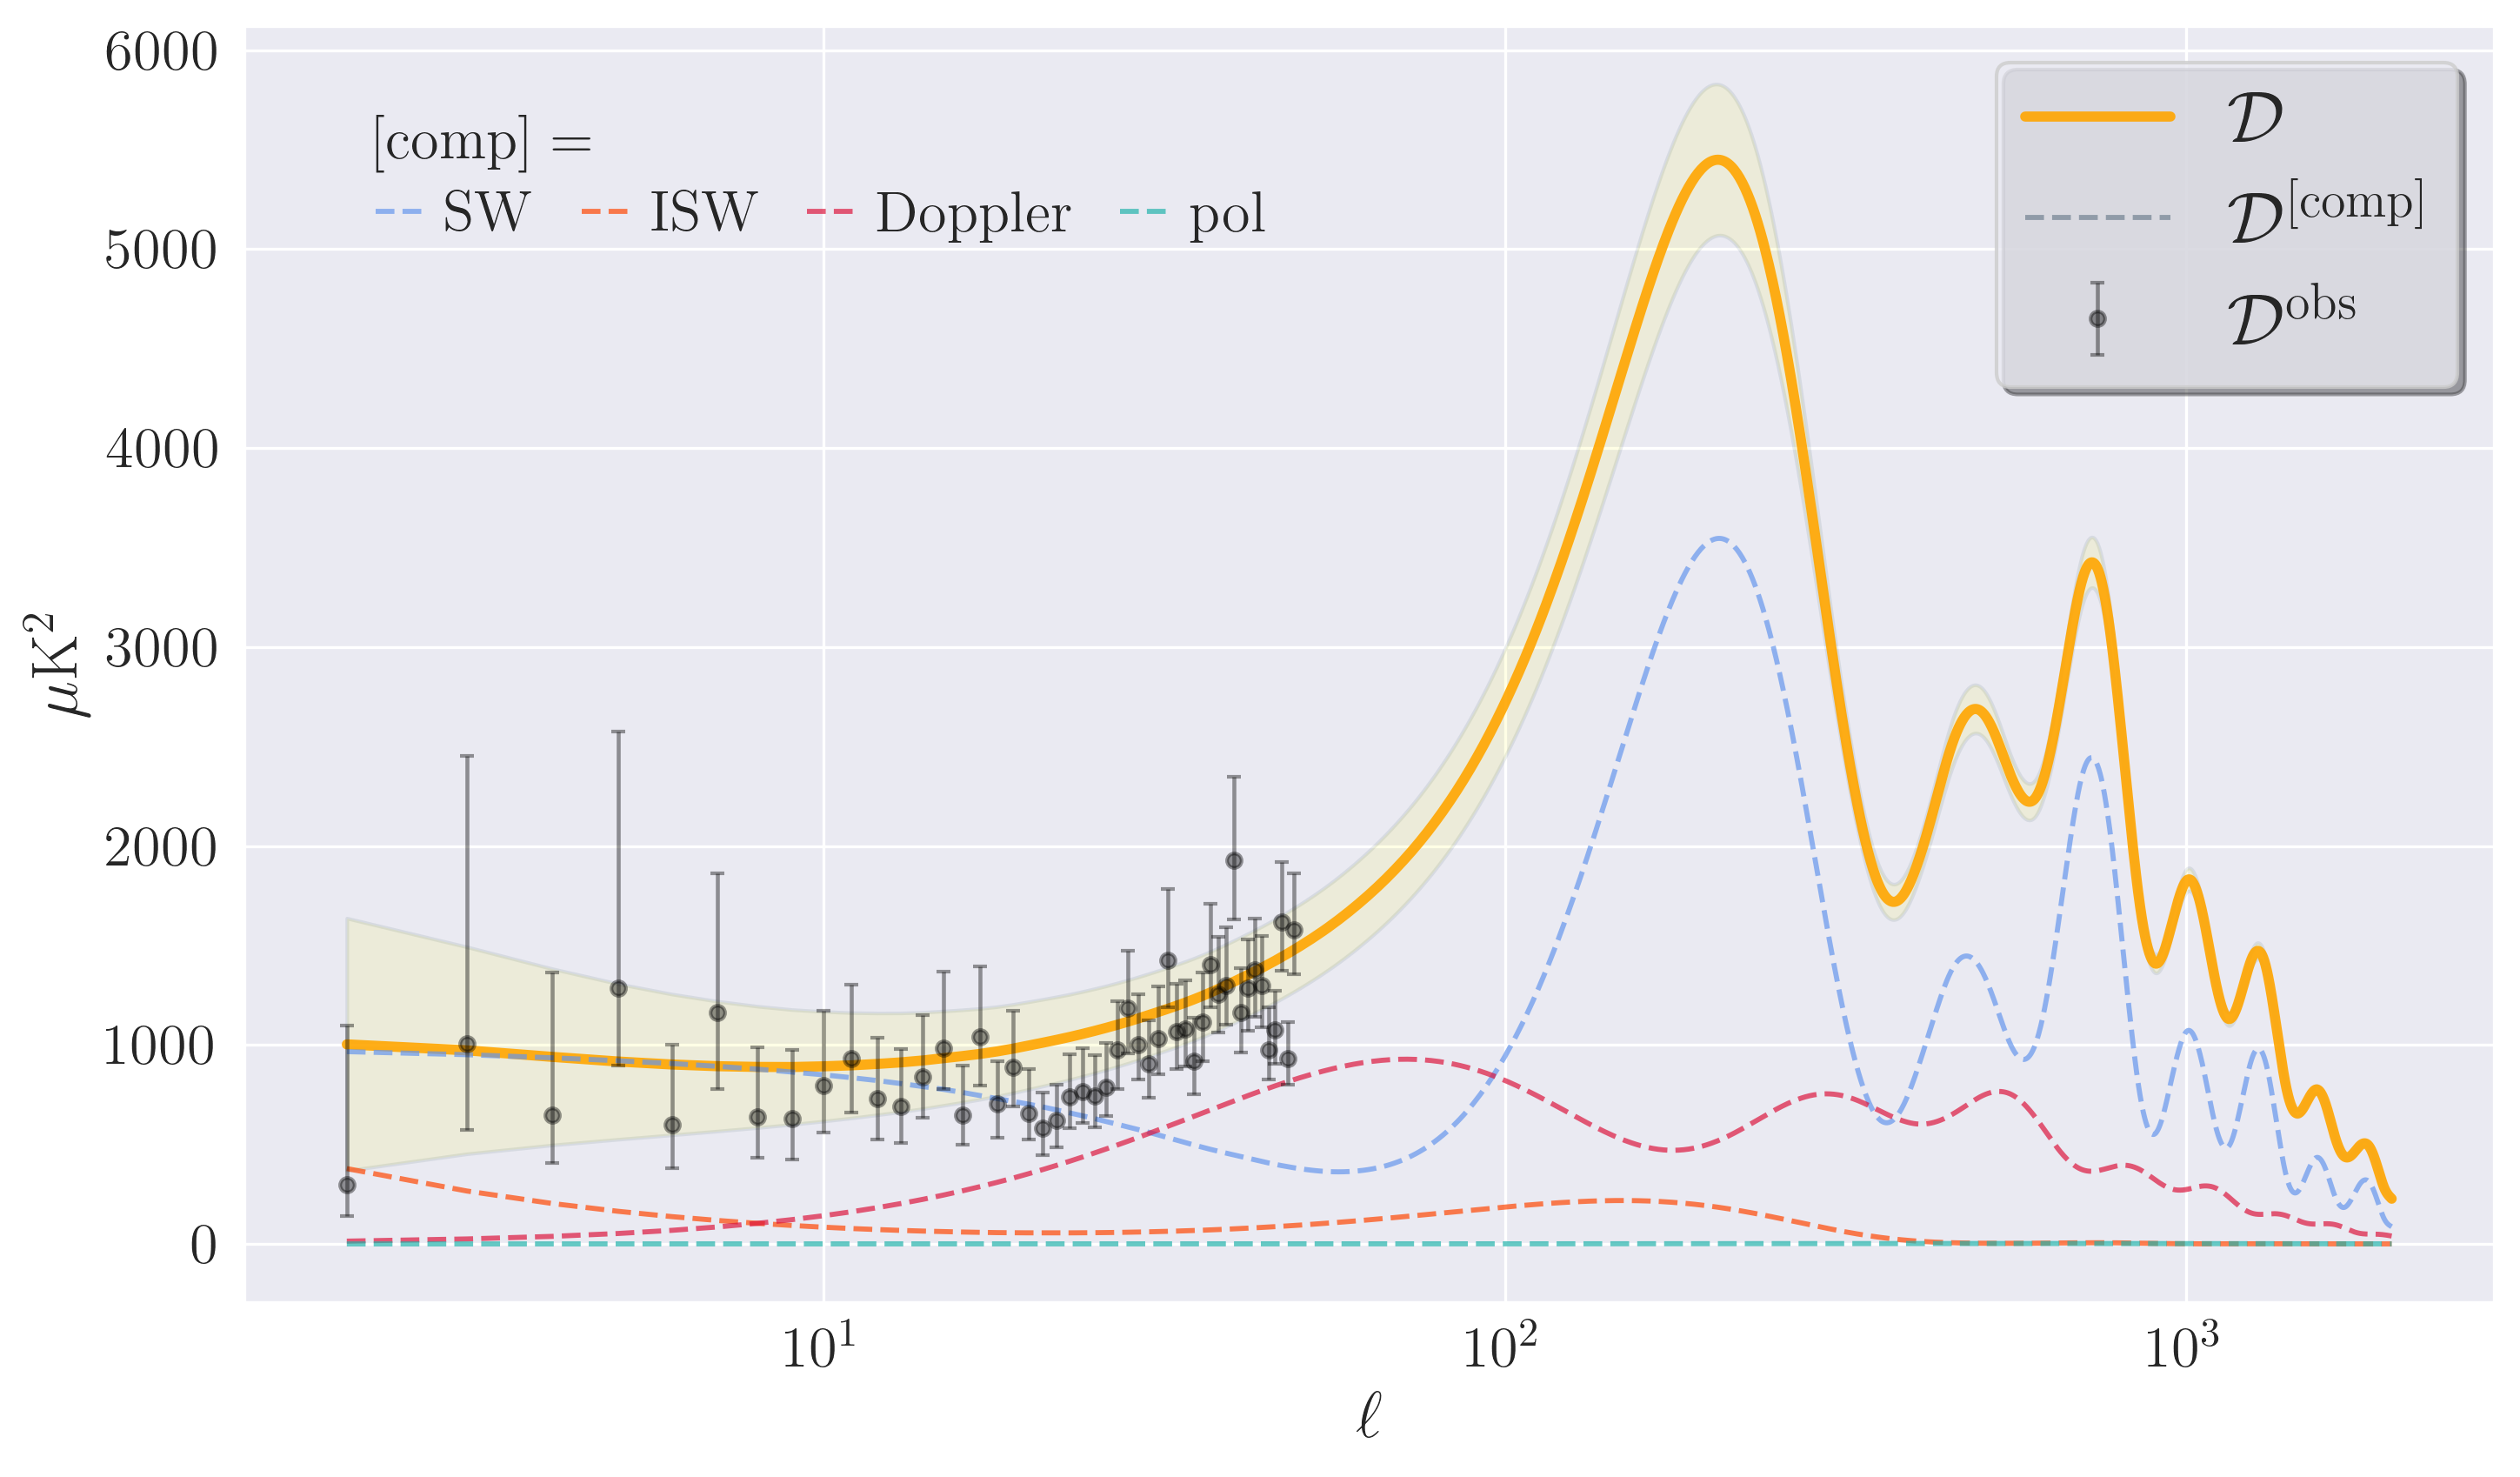
\includegraphics[width=\linewidth]{milestone4/CMB_power_spectrum.png} 
    \caption{The scaled CMB power spectrum $D(\ell)$ as function of multipole moment $\ell$. The shaded region represents the fundamental cosmic variance.} 
\label[fig]{mil4:res:fig:CMB_power}
\end{figure}

In figure~\cref{mil4:res:fig:matter_power} is plotted the total matter power spectrum. Observational data from~\citet{wmap_act} and \textcolor{blue}{CITE} is shown in the same figure. Discrepancy is significantly larger for smaller scales.
\begin{figure}[!ht]
    \centering
    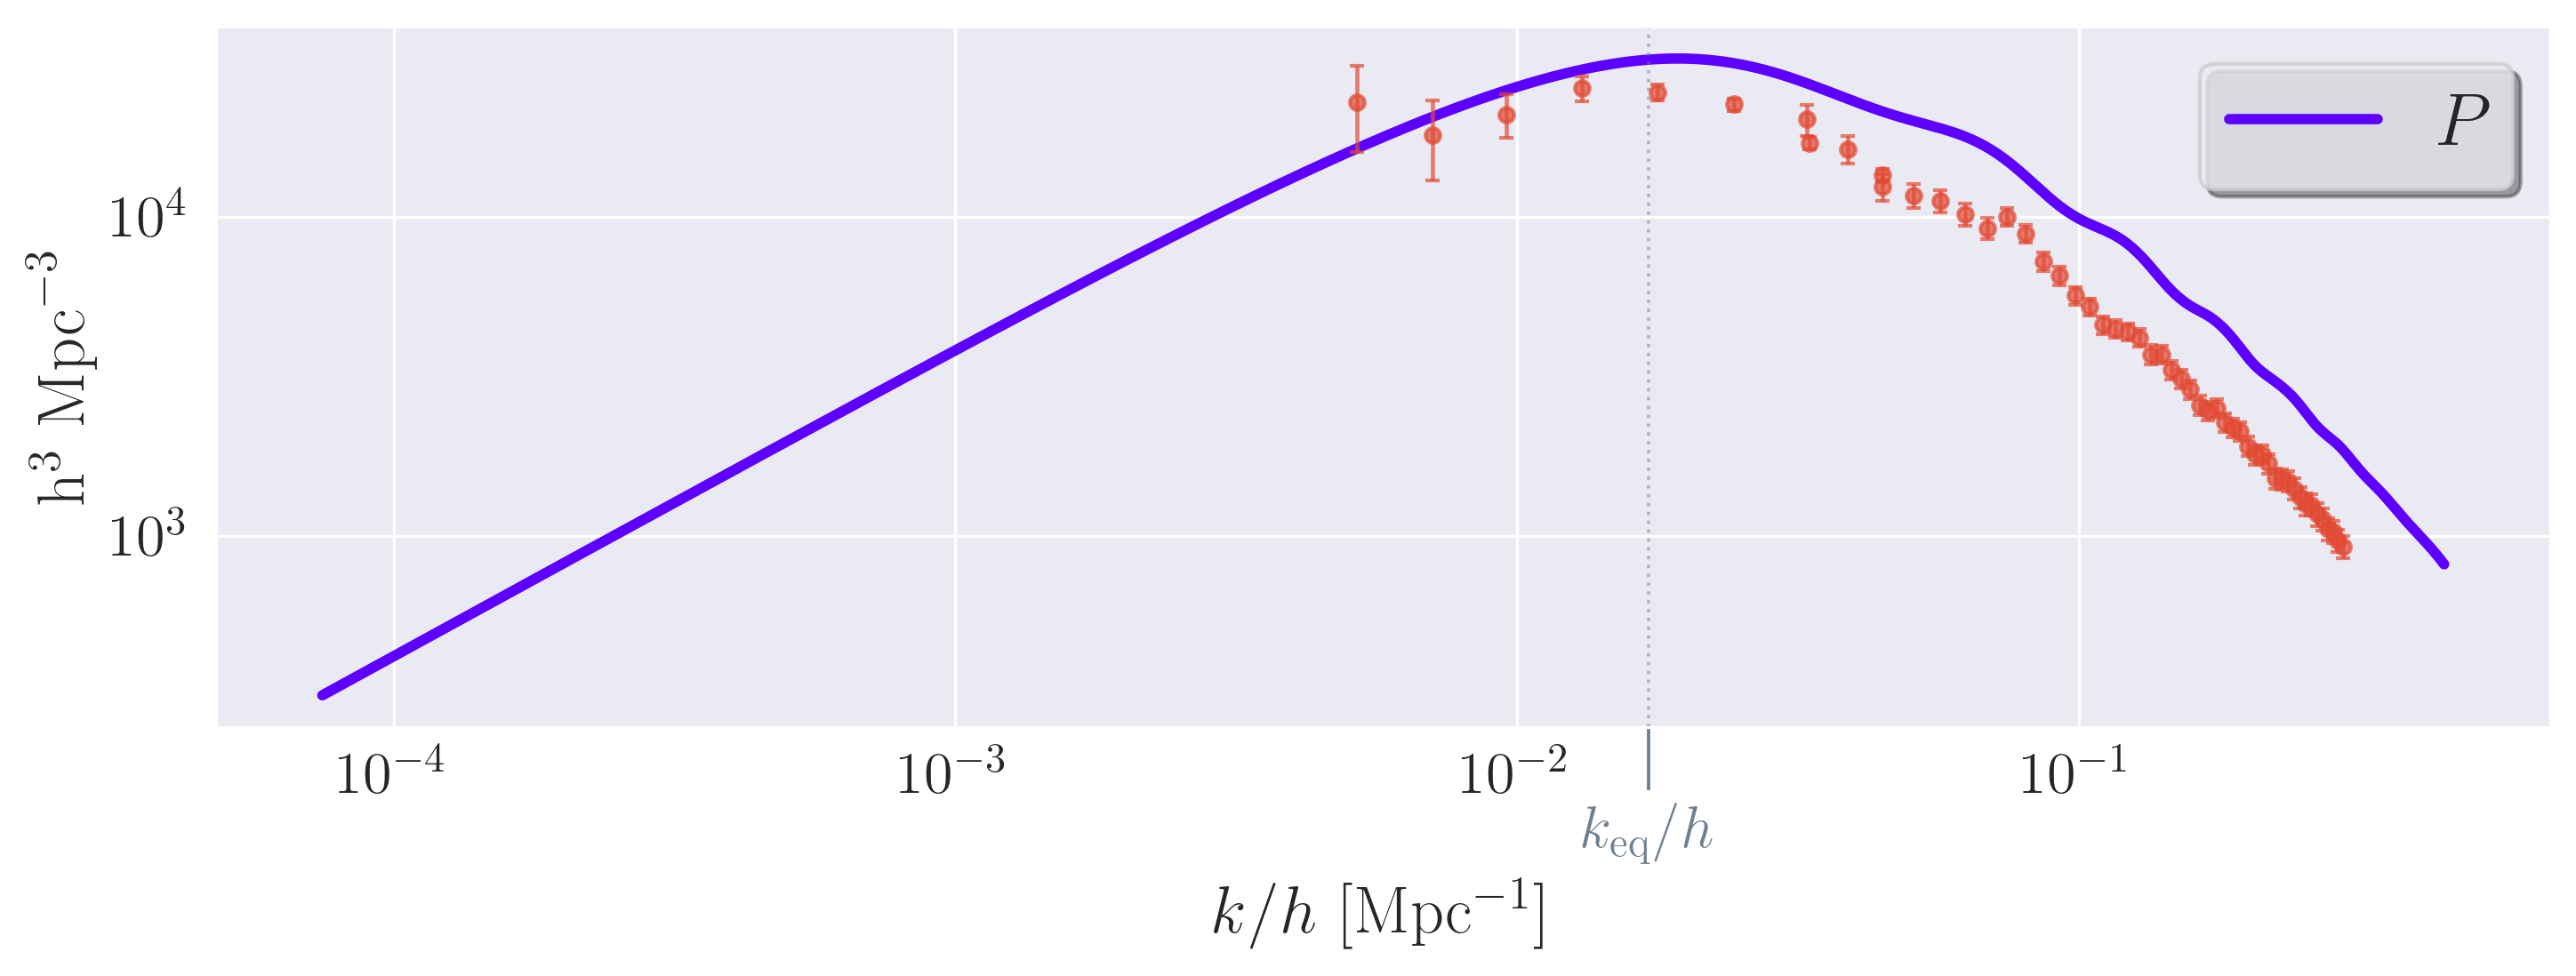
\includegraphics[width=\linewidth]{milestone4/matter_power_spectrum.png} 
    \caption{The total matter power spectrum $P(k)$ as function of wavenumber $k$. Both axes are logarithmic. The equality scale $k\ped{eq}$ is demonstrated by a vertical dotted line.} 
\label[fig]{mil4:res:fig:matter_power}
\end{figure}